%%%%%%%%%%%%%%%%%%%%%%%%%%%%%%%%%%%%%%%%%%%%%%%%%%%%%%%%%%%%%
\section{Docker Image for Oscillating Neutrino Spectra}\label{sec:apdx_nu_spec}
%%%%%%%%%%%%%%%%%%%%%%%%%%%%%%%%%%%%%%%%%%%%%%%%%%%%%%%%%%%%%
\lstinputlisting[language=bash]{appendices/Dockerfile.txt}

\clearpage

%%%%%%%%%%%%%%%%%%%%%%%%%%%%%%%%%%%%%%%%%%%%%%%%%%%%%%%%%%%%%
\section{Spline Fitting Statuses} \label{sec:apdx_nu_splines}
%%%%%%%%%%%%%%%%%%%%%%%%%%%%%%%%%%%%%%%%%%%%%%%%%%%%%%%%%%%%%

\begin{figure}[ht]
    \centering{
        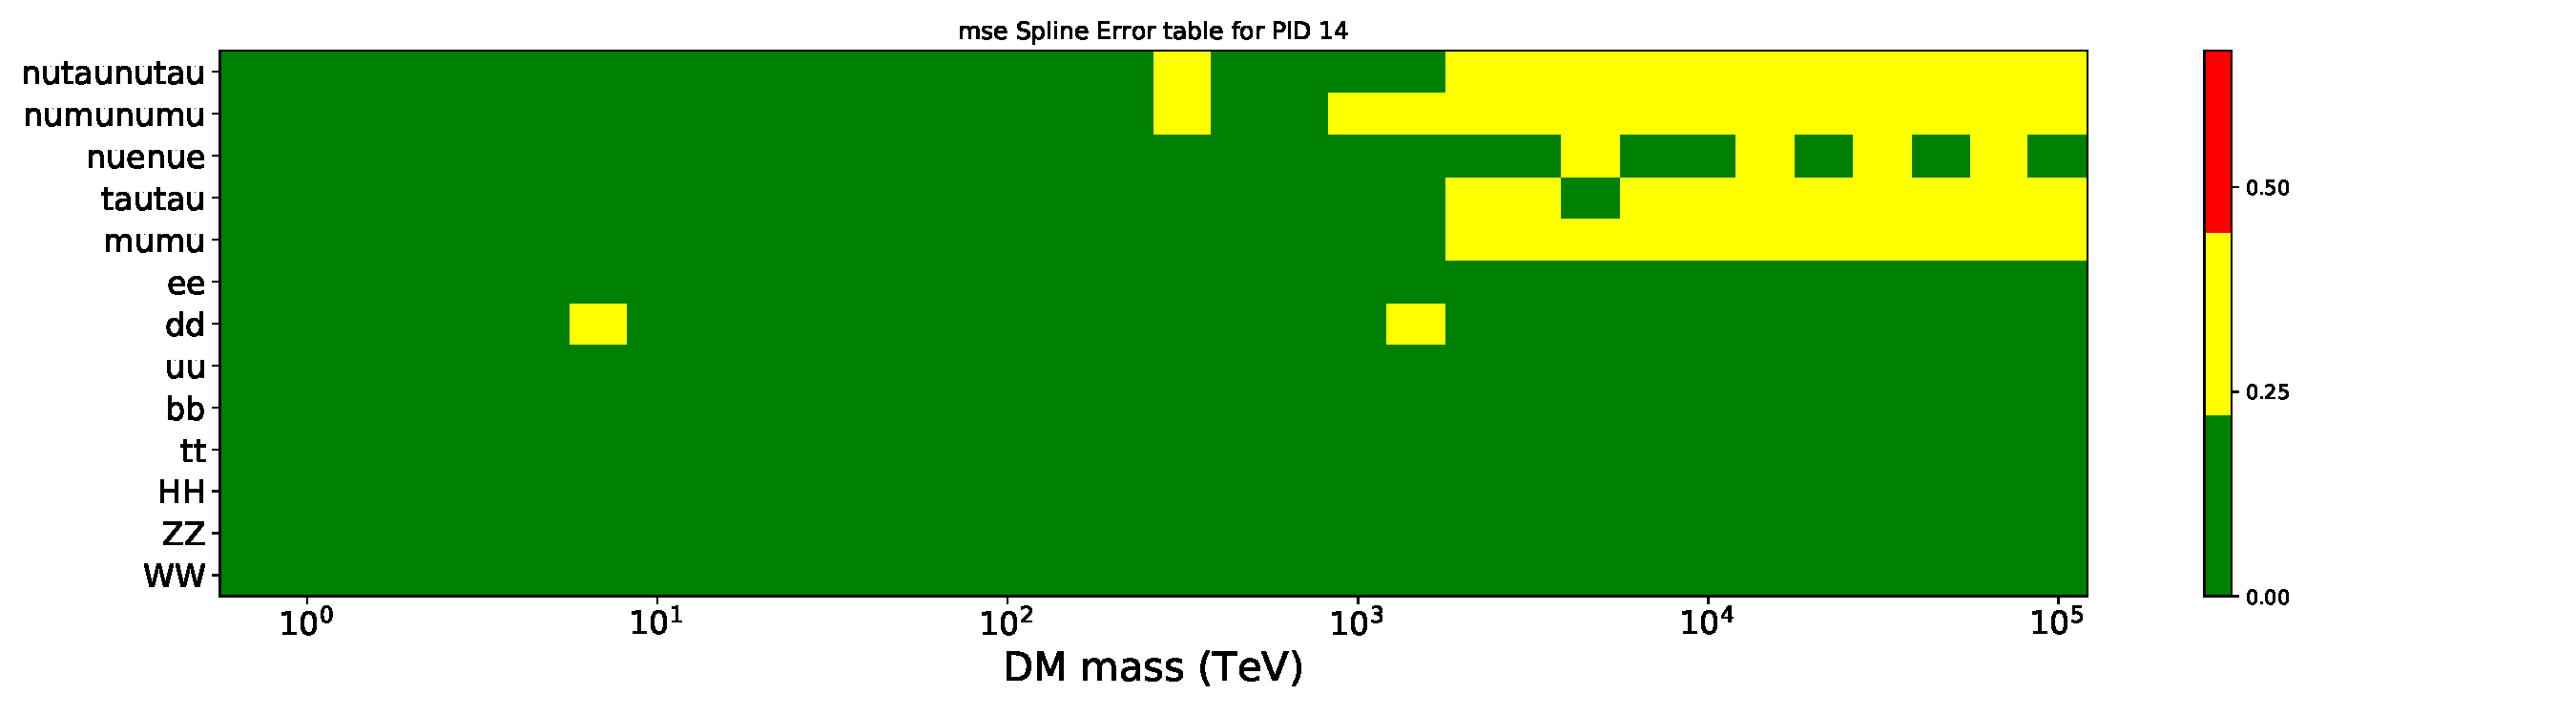
\includegraphics[scale=0.32]{figures/ic_DM/PID14_mse_error_chart.pdf}
        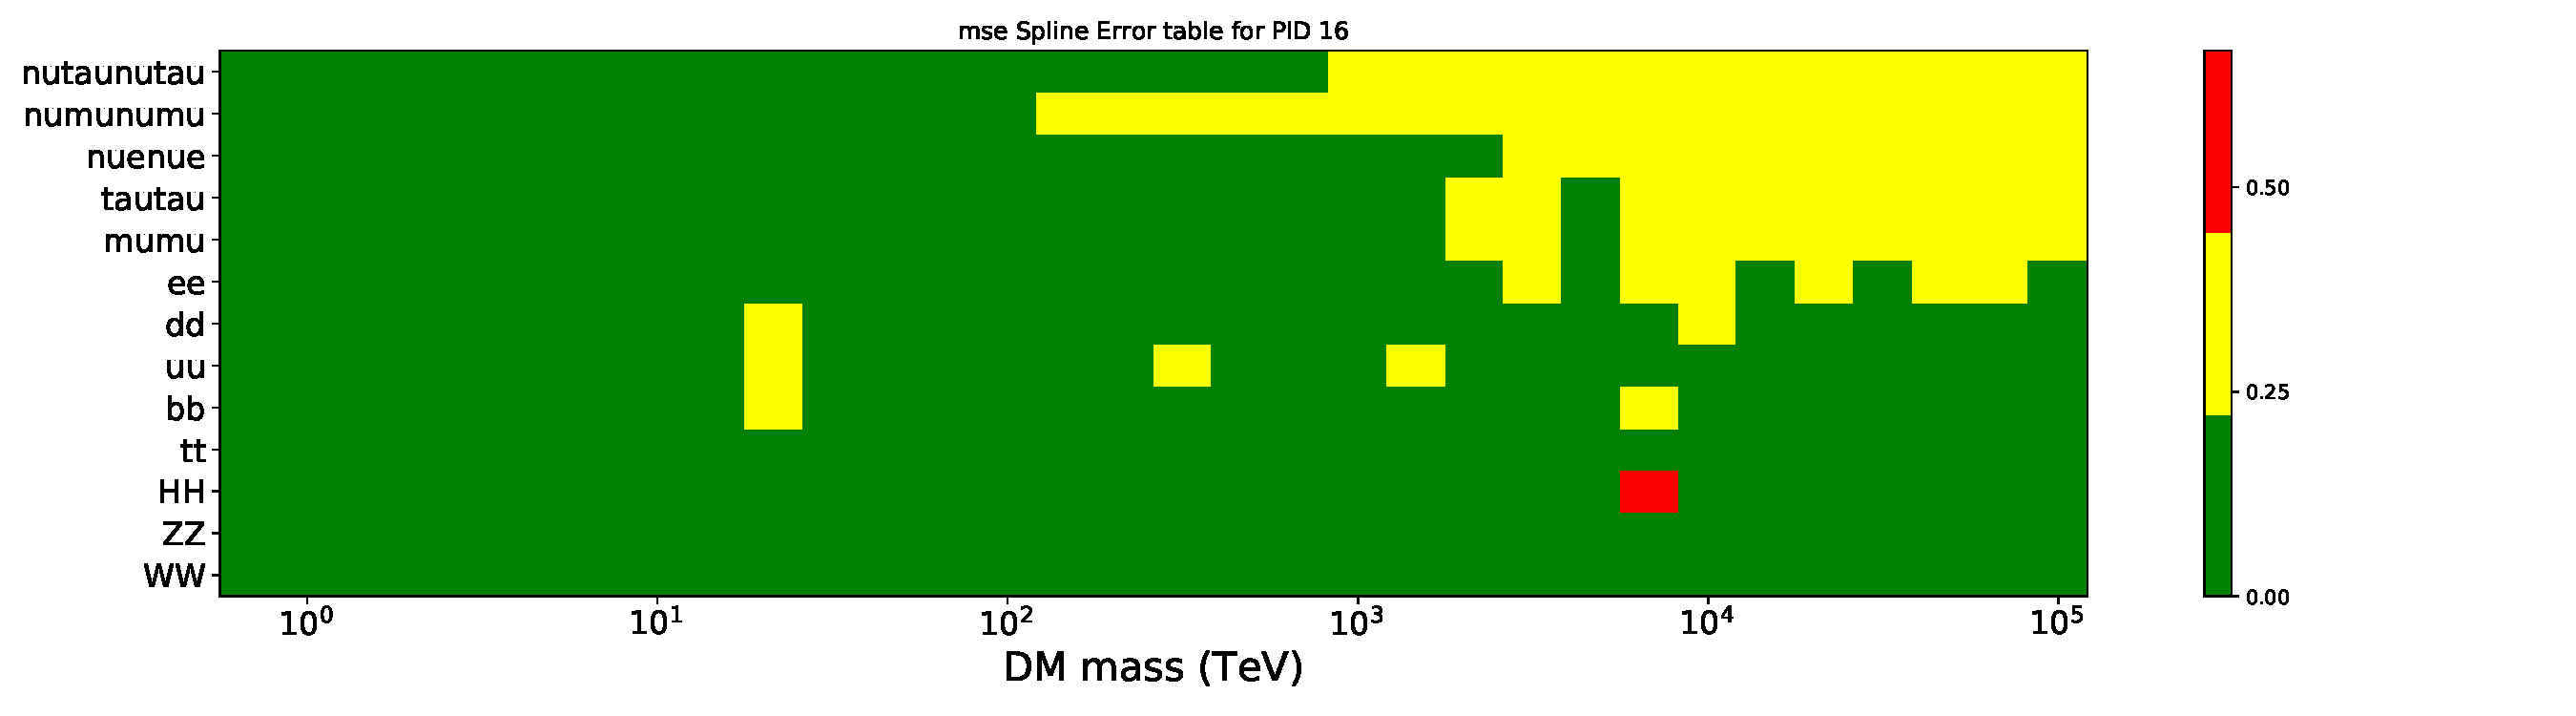
\includegraphics[scale=0.32]{figures/ic_DM/PID16_mse_error_chart.pdf}
    }
    \caption{Current status of spline tables according to contraints defined by \cref{tab:spline_tolerance}. Green splines are splines that passed under the GOOD tolerance. Yellow are splines that are OK. Red are splines that FAIL. All yellow splines were inspected individually before running the analysis. Splines were made for the $\mu$ (PID 14; top panel) flavor and $\tau$ (PID 16; bottom panel) neutrino flavors.}
    \label{fig:apdx_nu_splines}
\end{figure}

\clearpage
%%%%%%%%%%%%%%%%%%%%%%%%%%%%%%%%%%%%%%%%%%%%%%%%%%%%%%%%%%%%%
\section{Segue 1 And Ursa Major II Signal Recovery} \label{sec:apdx_TS_per_src}
%%%%%%%%%%%%%%%%%%%%%%%%%%%%%%%%%%%%%%%%%%%%%%%%%%%%%%%%%%%%%
 \tmpfig{Fill this out eventually. I think I want all the plots generated first}